\chapter{Quantum Monte-Carlo Methods} \label{chp:methods}
\epigraph{Great quote.}{Author}
\begin{figure}[H]
	\centering
	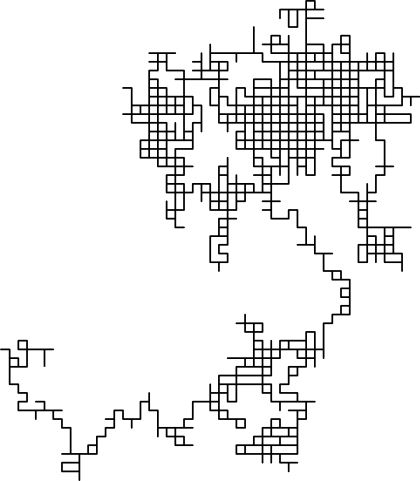
\includegraphics[scale=0.4]{Images/random_walk.png}
	\caption{Random walk on a two-dimensional grid.\\ © Copyright wikipedia.org.}
\end{figure}

Quantum Monte-Carlo methods (QMC) is a bunch of methods that attempt to solve the Schrödinger equation using stochastic Monte-Carlo integration. They all seek to evaluate the multi-dimensional integral arising from the Schrödinger equation,
\begin{equation}
E_0= \mel{\Psi_0}{\hat{\mathcal{H}}}{\Psi_0}= \frac{\int d\bs{r}\Psi_0(\bs{r})^*\hat{\mathcal{H}}\Psi_0(\bs{r})}{\int d\bs{r}\Psi_0(\bs{r})^*\Psi_0(\bs{r})},
\label{eq:schrodingergroundstate}
\end{equation}
which provides the ground state energy expectation value for the exact ground state wave function $\Psi_0$. As aforementioned, this integral is analytically infeasible for more or less all systems of interest, rising the need of numerical methods like QMC.

In Monte-Carlo integration, we use random number to evaluate integrals numerically. Typically, the we want to estimate an expectation value $\langle\mathcal{O}\rangle$ by approximating the definition integral with a dense sum,
\begin{equation}
\langle \mathcal{O}\rangle\equiv\int_{-\infty}^{\infty}d\bs{r}P(\bs{r})\hat{\mathcal{O}}(\bs{r})\approx\frac{1}{M}\sum_{i=1}^M\hat{\mathcal{O}}(\bs{r}_i)
\label{eq:montecarlointegration}
\end{equation}
where $M$ is the number of \textit{Monte-Carlo cycles} and the coordinates $\bs{r}_i$ are drawn randomly from the probability density function $P(\bs{r})$.

A great advantage of the QMC methods, is that we obtain approximative ground state wave functions when solving equation \eqref{eq:schrodingergroundstate}, which by the fourth postulate of quantum mechanics let us estimate ground state expectation values associated with other operators as well. 

Two widely popular QMC methods are the variational Monte-Carlo method (VMC) and the diffusion Monte-Carlo method (DMC), where the former is arguably the simplest of all the QMC methods. It attempts to directly solve the integrals in equation \eqref{eq:schrodingergroundstate} by varying parameters, with the support of the variational principle presented in section \ref{sec:variationalprinciple}. This makes VMC a relatively computationally cheap method, but the performance is not in the league of the best methods.

DMC, on the other hand, is computationally expensive, but is also potentially numerically exact, making it a preferred method when high accuracy is needed. At first glance it might seems like a tradeoff where VMC is used when computational time is more important than the accuracy and DMC is used when the opposite is true. However, DMC requires a wave function input which is close to the exact wave function, forcing us to first run VMC to obtain this wave function before the DMC machinery can be started.

As VMC is our main focus in this work, it will be explained thoroughly in this chapter together with common sampling techniques. In the end we will briefly explain the idea behind the DMC method, but since this method is not implemented it will not be in our main focus.

\section{Variational Monte-Carlo} \label{subsec:vmc}
The variational Monte-Carlo method (hereafter VMC) is today widely used when it comes to the study of ground state properties of quantum many-body systems. It makes use of Markov chain Monte-Carlo methods, often abbreviated MCMC, where the particles are assumed to be moving in Markov chains controlled by Monte-Carlo simulations. Going back to the variational principle in equation \eqref{eq:variationalprinciple}, one observes that by choosing an approved wave function, one gets an energy larger or equal to the ground state energy. \bigskip

Before we present the mathematical framework of the method, we will restate the two big problems in many-body physics, mentioned in the introduction:
\begin{enumerate}
	\item The many-body energy expectation value is analytically infeasible
	\item The correct many-body wave function is generally unavailable
\end{enumerate}

\subsection{Approaching the first problem}
Let us first address the first problem, which often is considered as the root of all evil in many-body physics. In chapter \ref{chp:quantum}, we saw that the two-body interaction term makes the integral impossible to solve for many particles, such that we need to rely on numerical methods. 

In VMC, we start with a trial wave function guess $\Psi_T(\bs{r};\bs{\theta})$ where the parameters $\bs{\theta}$ are varied to minimize the energy. According to the variational principle, the obtained energy will always be higher or equal to the true ground state energy, where the equality is the case if and only if the wave function is the exact ground state wave function. Denoting the exact ground state energy by $E_0$ and the obtained energy as $E$, we can summarize this by
\begin{equation}
E_0 \leq E = \frac{\int d\bs{r}\Psi_T(\bs{r})^*\hat{\mathcal{H}}\Psi_T(\bs{r})}{\int d\bs{r}\Psi_T(\bs{r})^*\Psi_T(\bs{r})}.
\end{equation}
Furthermore, the integral can be written on the form of a general expectation value
\begin{equation}
E = \int d\bs{r} P(\bs{r}) E_L(\bs{r})
\end{equation}
defining the local energy as
\begin{equation}
E_L(\bs{r})\equiv\frac{1}{\Psi_T(\bs{r})}\hat{\mathcal{H}}\Psi_T(\bs{r})
\label{eq:local energy}.
\end{equation}
$P(\bs{r})$ is called the probability density function (PDF), and was first presented in equation \eqref{eq:pdf}, and in a more general scheme the PDF reads
\begin{equation}
P(\bs{r})=\frac{|\Psi_T(\bs{r})|^2}{\int d\bs{r}|\Psi_T(\bs{r})|^2}.
\label{eq:probvmc}
\end{equation}
Since the energy expectation value now is on a form of a general expectation value, we can use the approximation set up by Monte-Carlo integration in equation \eqref{eq:montecarlointegration}, yielding 
\begin{equation}
E \approx \frac{1}{M}\sum_{i=1}^ME_L(\bs{r}_i) \label{eq:energysum}.
\end{equation}
We recall that the local energies $E_L(\bs{r}_i)$ are evaluated with particle configurations $\bs{r}_i$ drawn from the PDF $P(\bs{r})$. In this manner the obtained energy is guaranteed to approach the exact energy as the number of Monte-Carlo cycles, $M$, increases. Actually the standard error goes as $\mathcal{O}(1/\sqrt{M})$, making the method pretty accurate for large numbers of cycles. In the limit $M\rightarrow\infty$, the error goes to zero,
\begin{equation}
\langle E_L\rangle=\lim_{M\to\infty} \frac{1}{M}\sum_{i=1}^ME_L(\bs{r}_i),
\end{equation}
indicating the desire of largest number of cycles. This is associated with a zero-variance property governing the VMC method, stating that the variance in the true ground state should be zero. For more statistical details, see \cite{deb_variational_2014}.

\subsection{Approaching the second problem}
So far so good, but how do we attack the second problem stated above? One of the big strengths of VMC, as aforesaid, is that we obtain an approximative wave function meanwhile the energy expectation value is calculated. If we go back to equation \eqref{eq:probvmc}, we see that a PDF is required in order to estimate the energy, 

\subsection{Common extensions}
This finalizes the essential theory behind the VMC method. However, a sampling algorithm is needed to draw samples randomly from $P(\bs{r})$, and in section \ref{sec:metropolis} some popular sampling techniques are described. Before we jump into this field, we will discuss some usual extensions and improvements to the VMC method.

Initially, the particle configuration $\bs{r}$ might not be representative for a configuration in equilibrium, making the first cycles a poor estimate of the expectation value. An easy fix to this problem is to basically ignore the first sampling period, known as the \textit{burn-in period}. With this in mind, we implement an equilibriation fraction describing the fraction of the total number of cycles that is used in the burn-in period. When running multiple parallel processes, the burn-in period should be the same for all the processes.

We also have a technique called \textit{thinning}, which means picking every $n$'th sample in the chain and ignore the rest. This is shown to give a more or less identical expectation value and makes the program less memory-requiring, but due to worse statistics, this should be avoided as long as the computer does not lack memory. 

\section{The Metropolis algorithm} \label{sec:metropolis}
Metropolis sampling is a Markov chain Monte-Carlo method, which generates a Markov chain using a proposal density for new steps, and the method also rejects unsatisfying moves. In its most simple form, a particle is moved in a random direction, which was the original method invented by Metropolis et.al. back in 1953. \cite{metropolis_equation_1953} Later, the method was improved by Hastings et.al., giving rise to the more general Metropolis-Hastings algorithm. \cite{hastings_monte_1970}
The genius of the Metropolis algorithm, is that the acceptance of a move is not based on the probabilities themselves, but the ratio between the new and the old probabilities. In that way, we avoid calculating the sum over all probabilities, which is often computational intractable.

We will first discuss Markov chains in general, before we connect them to the original Metropolis algorithm, henceforth called \textit{brute-force sampling}, and then the Metropolis-Hastings algorithm, also called \textit{importance sampling}.

If we denote $\bs{r}$ as the current state, and $\bs{r}'$ as the proposed state, we have a transition rule $P(\bs{r}'|\bs{r})$ for going from $\bs{r}$ to $\bs{r}'$ and a transition rule $P(\bs{r}|\bs{r}')$ for going the opposite way. If we then assume that the rules satisfy \textit{ergodicity} and \textit{detailed balance}, we have the following relationship:
\begin{equation}
P(\bs{r}'|\bs{r})P(\bs{r})=P(\bs{r}|\bs{r}')P(\bs{r}'),
\end{equation}
which is actually a restatement of Bayes' theorem presented in section \ref{sec:bayes}.

The next step is to rewrite the transition rules in terms of a proposal distribution $T(\bs{r}'|\bs{r})$ and an acceptance probability $A(\bs{r}',\bs{r})$,
\begin{equation}
P(\bs{r}'|\bs{r})=T(\bs{r}'|\bs{r})A(\bs{r}',\bs{r}).
\end{equation}
In order to satisfy the detailed balance, we need to choose $A(\bs{r}',\bs{r})$ such that
\begin{equation}
A(\bs{r}',\bs{r})=\text{min }\left[1,\frac{T(\bs{r}|\bs{r}')P(\bs{r}')}{T(\bs{r}'|\bs{r})P(\bs{r})}\right],
\label{eq:acceptance}
\end{equation}
since $A$ cannot be larger than 1. We want to accept a move with probability $A(\bs{r}',\bs{r})$. One way to do that is to draw a number from a uniform distribution between 0 and 1. If this number is lower than the acceptance, the move should be accepted. Otherwise it will be rejected.

\subsection{Brute-force sampling}
In its simplest form, the move is proposed randomly both in magnitude and direction. Mathematically, we can write this as
\begin{equation}
\bs{r}'=\bs{r}+sd\bs{r}
\end{equation}
where $s$ is a random number which determines the distance to move and $d\bs{r}$ is a random direction (typically which particle to move). We obtain the naive acceptance probability when requiring $T(\bs{r}'|\bs{r})=T(\bs{r}|\bs{r}')$, such that the it simplifies to
\begin{equation}
A(\bs{r}',\bs{r})=\text{min }\left[1,\frac{P(\bs{r}')}{P(\bs{r})}\right].
\end{equation}

However, with this approach a lot of moves will be rejected, which results in a significant waste of computing power. A better method is \textbf{importance sampling}.

\subsection{Importance sampling} \label{sec:importancesampling}
Importance sampling is a more intelligent sampling method than the brute-force sampling, since the new position is based on an educated guess. To understand how it works, we need to take a quick look at diffusion processes. We start from the Fokker-Planck equation,
\begin{equation}
\frac{\partial P(\bs{r},t)}{\partial t}=D\nabla\left(\nabla-\bs{F}\right)P(\bs{r},t)
\end{equation}
which describes how a probability distribution $P(\bs{r},t)$ evolves in appearance of a drift force $\bs{F}$. In the case $\bs{F}=0$, the equation reduces to the diffusion equation with $D$ as the diffusion constant. This simplifies to $D=1/2$ in atomic units. 

The Langevin equation states that a diffusion particle tends to move parallel to the drift force in the coordinate space, but because of a random variable $\bs{\eta}$ this is not always true. The equation reads
\begin{equation}
\frac{\partial \bs{r}(t)}{\partial t}=D\bs{F}(\bs{r}(t))+\bs{\eta}.
\label{eq:langevin}
\end{equation}
Given a position $\bs{r}$, the new position $\bs{r}'$ can be be found by applying forward-Euler on equation \eqref{eq:langevin},
\begin{equation}
%\bs{r}'=\bs{r}+D\bs{F}(\bs{r})\Delta t + \bs{\xi}\sqrt{\Delta t}
\end{equation}
where $\Delta t$ is a fictive time step and $\bs{\xi}$ is a Gaussian random variable. The next thing we want to find, is an expression for the drift force $\bs{F}$ which makes the system converge to a stationary state. 

A stationary state is found when the probability density $P(\bs{r})$ is constant in time, i.e, when the left-hand-side of Fokker-Planck is zero. In that case, we can write the equation as
\begin{equation}
\nabla^2P(\bs{r})=P(\bs{r})\nabla\bs{F(\bs{r})}+\bs{F(\bs{r})}\nabla P(\bs{r}).
\end{equation}
In the next, we assume that the drift force takes the form $\bs{F(\bs{r})}=g(\bs{r})\nabla P(\bs{r})$, since the force should point to a higher probability. We can then go further and write
\begin{equation}
\nabla^2 P(\bs{r})\big(1-P(\bs{r})g(\bs{r})\big)=\nabla\big(g(\bs{r})P(\bs{r})\big)\nabla P(\bs{r})
\end{equation}
which is satisfied when $g(\bs{r})=1/P(\bs{r})$. We then get the drift force 
\begin{equation}
\bs{F}(\bs{r})=\frac{\nabla P(\bs{r})}{P(\bs{r})}=2\frac{\nabla\Psi_T(\bs{r})}{\Psi_T(\bs{r})}=2\nabla\ln\Psi_T(\bs{r}),
\end{equation}
which is also known as the \textit{quantum force}.

\IncMargin{1em}
\begin{algorithm} [t]
	\SetAlgoLined
	\Parameter{$\Delta t$: Fictive time step}
	\Data{$\bs{r}'$: Initial particle positions}
	\Require{$\Psi_T(\bs{r})$: Initial trial wave function guess}
	\BlankLine
	$\bs{F}(\bs{r}')\leftarrow2(\nabla\Psi_T(\bs{r}'))/\Psi_T(\bs{r}')$ (Initialize the quantum force) \;
	$p(\bs{r}',\bs{r})\leftarrow1$ (Initialize the probability ratio) \;
	$g(\bs{r}',\bs{r},\Delta t)\leftarrow1$ (Initialize Green's function ratio) \;
	\While{not converged}{
		$\bs{r}\leftarrow\bs{r}'$ (Save current positions $\bs{r}'$ in a vector $\bs{r}$) \;
		$\bs{F}(\bs{r})\leftarrow\bs{F}(\bs{r}')$ (Save the current quantum force, $\bs{F}(\bs{r}')$, in a vector $\bs{F}(\bs{r})$) \;
		$p(\bs{r},\bs{r}')\leftarrow p(\bs{r}',\bs{r})$ (Save current probability ratio)\;
		$g(\bs{r},\bs{r}',\Delta t)\leftarrow g(\bs{r}',\bs{r},\Delta t)$ (Save the current Green's function ratio) \;
		\BlankLine
		$\bs{r}'\leftarrow\bs{r}+D\Delta t\bs{F}(\bs{r}) + \bs{\xi}\sqrt{\Delta t}$ (Update position based on the Langevin equation) \;
		$\bs{F}(\bs{r}')\leftarrow2\nabla\ln\Psi_T(\bs{r'})$ (Update the quantum force) \;
		$p(\bs{r}',\bs{r})=|\Psi_T(\bs{r}')|^2/|\Psi_T(\bs{r})|^2$ (Update the probability ratio) \;
		$g(\bs{r}',\bs{r},\Delta t)=G(\bs{r}',\bs{r},\Delta t)/G(\bs{r},\bs{r}',\Delta t)$ (Update the Green's function ratio) \;
		$w\leftarrow p(\bs{r}',\bs{r}) g(\bs{r}',\bs{r},\Delta t)$ (Calculate acceptance probability) \;
		$q\leftarrow\mathcal{U}(0,1)$ (Draw a random number between 0 and 1)\;
		\eIf{$w<q$}{
			$\bs{r}'\leftarrow\bs{r}$ (Reset positions)\;
			$\bs{F}(\bs{r}')\leftarrow\bs{F}(\bs{r})$ (Reset the quantum force) \;
			$p(\bs{r}',\bs{r})\leftarrow p(\bs{r},\bs{r}')$ (Reset the probability ratio)\;
			$g(\bs{r}',\bs{r},\Delta t)\leftarrow g(\bs{r},\bs{r}',\Delta t)$ (Reset the Green's function ratio) \;
		}
		{
			keep going\;
		}
	}
	\KwResult{The optimized trial wave function.}
	\caption{The Metropolis-Hastings algorithm. The positions are initialized randomly or was chosen by a previous sampling. The parameters are also usually initialized randomly or chosen by a parameter update. The Green's function ratio, $g$, can be evaluated efficiently using equation \eqref{eq:greensratio}, and the probability ratio $p$ can also often be found in a simple closed-form expression. The diffusion constant is $D=1/2$ in natural units. $\bs{\xi}$ is a random Gaussian variable. For more information, see section \ref{sec:importancesampling}}.
	\label{alg:hastings}
\end{algorithm}\DecMargin{1em}

The remaining part is how to decide if a proposed move should be accepted or not. For this, we need to find the sampling distributions $T(\bs{r}'|\bs{r})$ from equation \eqref{eq:acceptance}, which are just the solutions of the Fokker-Planck equation. The solutions read
\begin{equation}
G(\bs{r},\bs{r}',\Delta t)\propto\exp\Big(-\big(\bs{r}-\bs{r}'-D\Delta t\bs{F}(\bs{r})\big)^2/4D\Delta t\Big)
\end{equation}
which is called Green's functions. They correspond to the normal distribution $\mathcal{N}(\bs{r}|\bs{r}'+D\Delta t \bs{F}(\bs{r}),2D\Delta t)$. The acceptance probability for importance sampling can finally be written as
\begin{equation}
A(\bs{r}'|\bs{r})=\text{min }\left[1,\frac{G(\bs{r},\bs{r}',\Delta t)P(\bs{r}')}{G(\bs{r}',\bs{r}, \Delta t)P(\bs{r})}\right],
\end{equation}
where the marginal probabilities are still given by equation \eqref{eq:probvmc}. 

As a summary, we set up the actual algorithm, known as Metropolis-Hasting's algorithm, see algorithm \eqref{alg:hastings}. In that algorithm, we write the position update in a general form, where we allow updating all the particles at the same time. However, often one ends up moving only a particle at each time step, as this make some advantageous optimization schemes possible. 

The ratio between the new and old Green's function can be expressed in the elegant form 
\begin{equation}
g(\bs{r}',\bs{r},\Delta t)\equiv\frac{G(\bs{r}',\bs{r},\Delta t)}{G(\bs{r},\bs{r}',\Delta t)}=\exp((\bs{r}'-\bs{r})\cdot(\bs{F}(\bs{r})-\bs{F}(\bs{r}'))/2)
\label{eq:greensratio}
\end{equation}
which can be evaluated very efficiently. Also the probability ratios can be computed in an efficient way for many trial wave functions $\Psi_T(\bs{r})$, in particular when the wave function is on an exponential form. In chapter \ref{chp:WFE}, we find closed-form expressions for
\begin{equation}
p(\bs{r}',\bs{r})\equiv\frac{P(\bs{r}')}{P(\bs{r})}=\frac{|\Psi_T(\bs{r}')|^2}{|\Psi_T(\bs{r})|^2}
\end{equation}
for all the wave function elements of interest, also the elements based on restricted Boltzmann machines. Additionally, closed-form expressions fo $\nabla\ln\Psi_T(\bs{r})$ are found, which are needed for the quantum force computations as well as the kinetic energy computations. 

\subsection{Gibbs sampling}
In the machine learning community, Gibbs sampling is widely used when it comes to training Boltzmann machines. It is popular partly because it does not require any "tuning". It is an instance of the Metropolis-Hastings algorithm, and is therefore another Markov chain Monte-Carlo method. In the Metropolis sampling, we have seen that some moves will be rejected, but in Gibbs sampling all the moved are accepted, which means that the we do not "waste" computations. 

The point of Gibbs sampling is that given a multivariate distribution it is simpler to sample from a conditional distribution than to marginalize by integrating over a joint distribution. This is the reason why we do not need the marginal distributions in Gibbs sampling, but rather the conditional distributions. In the most general, Gibbs sampling proposes a rule for going from a sample $\bs{x}^{(i)}=(x_1^{(i)},x_2^{(i)},\hdots,x_n^{(i)})$ to another sample $\bs{x}^{(i+1)}=(x_1^{(i+1)},x_2^{(i+1)},\hdots,x_n^{(i+1)})$, similar to the Metropolis algorithm. However, in Gibbs sampling the transition from $x_j^{(i)}$ to $x_j^{(i+1)}$ is performed according to the conditional distribution specified by
\begin{equation}
P\big(x_j^{(i+1)}|x_1^{(i+1)},\hdots,x_{j-1}^{(i+1)},x_{j+1}^{(i)},\hdots,x_n^{(i)}\big).
\end{equation}
The marginal distribution of a subset of variables can then be approximated by simply considering the samples for that subset of variables, ignoring the rest. 

For a restricted Boltzmann machine, this is a two-step sampling process, because of the latent variables, we use the conditional probabilities $P(\bs{r}|\bs{h})$ and $P(\bs{h}|\bs{r})$ to update the visible and hidden units respectively. For the restricted Boltzmann machine with Gaussian-binary units presented in section \ref{sec:RBM}, the conditional probability of $h_j=0$ given a set of visible nodes $\bs{x}$ is
\begin{equation}
P(h_j=0|\bs{x})=\frac{1}{1+\exp(b_j+\sum_{i=1}^Nx_iw_{ij}/\sigma^2)}
\end{equation}
and the corresponding conditional probability of $h_j=1$ is
\begin{equation}
P(h_j=1|\bs{x})=\frac{1}{1+\exp(-b_j-\sum_{i=1}^Nx_iw_{ij}/\sigma^2)},
\end{equation}
which is by the way the sigmoid function again. Note that $P(h_j=0|\bs{x})+P(h_j=1|\bs{x})=1$, indicating that a hidden node $h_j$ can only take 0 or 1, hence binary. When updating the hidden node, one typically calculate the sigmoid $P(h_j=1|\bs{x})$ and set $h_j$ to 1 if this probability is larger than 1/2, and set it to 0 otherwise. 

For the update of the visible nodes, we see from equation \eqref{eq:normal} that the visible nodes are chosen after the normal distribution,
\begin{equation}
P(x_i|\bs{h})=\mathcal{N}\Big(a_i+\sum_{j=1}^Hw_{ij}h_j,\sigma^2\Big)
\end{equation}
which introduce some stochasticity to the system. By going back and forth in the Boltzmann machine multiple times (a round trip corresponds to an iteration), the hope is that the expectation values can be approximated by averaging over all the iterations. 

As pointed out earlier, the Gibbs sampling will not be implemented in this work, but is described for completeness purposes. The reason for this, is that the method has not shown promising results for our specific problem, and we will instead rely on Metropolis sampling. We have already tested the Gibbs sampling in another similar project on small quantum dots \cite{nordhagen_computational_2018}, and so have others like Vilde Flugsrud \cite{flugsrud_vilde_moe_solving_nodate}. The results are similar and poor compared to the Metropolis-Hastings algorithm.

However, the Gibbs sampling method itself should not be underestimated. Carleo and Troyer showed its importance when solving the Ising model using a restricted Boltzmann machine and Gibbs sampling, and in traditional Boltzmann machines the Gibbs sampling is the preferred tool. \cite{carleo_solving_2017}

\section{Similarities between restricted Boltzmann machines and variational Monte-Carlo}
In chapter \ref{chp:systems}, we presented the relation between a quantum system and expressions of the Hamiltonian, which is the energy operator. In section \ref{sec:unsupervised}, we described how Boltzmann machines are defined and how one can find the energy of a Boltzmann machine. Further, we looked at the updating schemes, which for both cases corresponds to minimizing the cost function and maximizing the log-likelihood function. 

All in all, there are many similarities between the two methods. They are fundamentally related through Markov random fields, ...

\section{Diffusion Monte-Carlo}
Diffusion Monte-Carlo belongs to a class of projection and Green's function approaches. Consider the time-imaginary Schrödinger equation
\begin{eqnarray}
-\frac{\partial\Psi(\bs{r},\tau)}{\partial\tau}=(\mathcal{H}-E_T)\Psi(\bs{r},\tau)
\end{eqnarray}
where $\tau$ is the imaginary time and $E_T$ is an energy offset. If we first look at the equation with non-interacting particles, it contains basically only the kinetic energy term, 
\begin{equation}
\frac{\partial\Psi(\bs{r},\tau)}{\partial\tau}=\frac{1}{2}\nabla^2\Psi(\bs{r},\tau)
\end{equation}
which is really similar to the diffusion equation,
\begin{equation}
\frac{\partial\phi(\bs{r},t)}{\partial t}=D\nabla^2\phi(\bs{r},t)
\end{equation}
where $D$ is the diffusion constant set to $1/2$ in our calculations, no wonder why. The similarities between the imaginary time Schrödinger and the diffusion equation was noticed by Fermi already around 1945, and is what diffusion Monte-Carlo is based on \cite{metropolis_monte_1949,ceperley_quantum_1986}. 

A solution of the 


